\chapter{Optical lattices and the Bose-Hubbard model}

\NOTE{intro}

\label{sec:chapter_2}

\section{The Bose-Hubbard Model}

We consider a 3D lattice potential with cubic symmetry and spacing $d$:

\begin{equation}
    V(\bm{r})=V_{0}\left[\sin ^{2}\left(\frac{k_{d}}{2} x\right)+\sin ^{2}\left(\frac{k_{d}}{2} y\right)+\sin ^{2}\left(\frac{k_{d}}{2} z\right)\right] + V_{\mathrm{ext}} (x,y,z)
\end{equation}

\noindent where $k_d=\frac{2 \pi}{d}$ is the associated wavevector, $V_0$ the lattice amplitude. For convenience, $V_0$ is usually expressed in units of recoil energy $V_0 = s E_{\rm{r}}$ with $E_r=h^2/ 8 m d^2$. The term $V_{\mathrm{ext}} (x,y,z)$ denotes a harmonic potential related to the Gaussian shape of the lattice beams. For simplicity of calculations, we will only treat here the homogeneous case $V_{\mathrm{ext}} (x,y,z)=0$.

We consider an ensemble of $N$ atoms that interact with one another with the potential $U_{\rm{int}} ( \bm{r}_1, \bm{r}_2)$ loaded in the lattice potential $V(\bm{r})$. The Hamiltonian of the system writes:

\begin{equation}
    \hat{H}=\sum_{i=1}^{N} \frac{\bm{p}_{i}^{2}}{2 m}+\sum_{i=1}^{N} V\left(\bm{r}_{i}\right) + \sum_{i}^{N} \sum_{j>i}^{N} U_{\text{int}}\left(\bm{r}_{i}, \bm{r}_{j}\right)
    \label{eq:H_lattice_full}
\end{equation}

\subsubsection{Non-interacting lattice gas}

To begin, we will not consider interactions and study the simplified Hamiltonian:

\begin{equation}
    \hat{H}_0=\sum_{i=1}^{N} \frac{\bm{p}_{i}^{2}}{2 m}+\sum_{i=1}^{N} V\left(\bm{r}_{i}\right)
\end{equation}

\noindent As the Hamiltonian is separable along the 3 directions of space and the gas of atoms is non-interacting, we can simply work with the one-dimensional, single particle Hamiltonian:

\begin{equation}
    \hat{H}_1 = \frac{p_x}{2m} + \sin^2 \Big(\frac{k_d}{2} x \Big)
\end{equation}

\noindent To find the eigenstates of this Hamiltonian, we use the Bloch's theorem \cite{ashcroft1976solid}:

\begin{tcolorbox}[colback=red!5!white,colframe=red!75!black,title=\textbf{Bloch's theorem}]
\label{sec:bloch}
The eigenstates of a Hamiltonian corresponding to a spatially periodic potential $V(\bm{r})$ on a lattice $\mathcal{B}$ are Bloch waves $\psi_{\bm{q}}(\bm{r})$, product of a plane-wave $e^{i \bm{r}.\bm{q}}$ and a periodical function on $\mathcal{B}$, $u_{\bm{q}} (\bm{r})$.
\end{tcolorbox}

We therefore look eigenstates of the form:

\begin{equation}
    \psi_{n,q} (x)= e^{iqx} u_{n,q} (x)
    \label{eq:bloch_wave}
\end{equation}

\noindent with $n \in \N$ and $q \in \R$ the \textbf{quasi-impulsion}. As $E_n (q)$ is periodic $E_n (q+k_d)= E_n(q) \ \forall (n,q)$, we can restric the definition interval of $q$ to $[-k_d/2, k_d/2]$ which is called the \textbf{first Brillouin zone}. In order to determine the functions $u_{\bm{q}} (\bm{r})$, we inject equation \ref{eq:bloch_wave} in the eigenvalue equation to find that they must verify:

\begin{equation}
    \left[\frac{\left(p_{x}+\hbar q\right)^{2}}{2 m}+V_{0} \sin ^{2}\left(\frac{k_{a}}{2} x\right)\right] u_{n, q}(x)=E_{n}(q) u_{n, q}(x)
\end{equation}

The Bloch energy bands $E_{n}(q)$ and the Bloch functions $u_{n, q}(x)$ can be easily numerically calculated. We plot on Fig.-\ref{fig:bloch_bands} the first five energy bands as a function of $q$ in the first Brillouin zone for various values of the lattice amplitude $V_0$. Interestingly, we see that a gap appears between the different bands as we increase $V_0$. For a 3D lattice, the total energy is the sum of the energies along each direction of the lattice. The first excited band then corresponds to two 1D lowest energy bands and one 1D excited band. In order for the gap to appear, the lattice amplitude must be above $V_0 \simeq 2.2 \ E_{\mathrm{r}}$, whereas it is present at all values of $V_0$ in the 1D case.

\begin{figure}
    \centering
    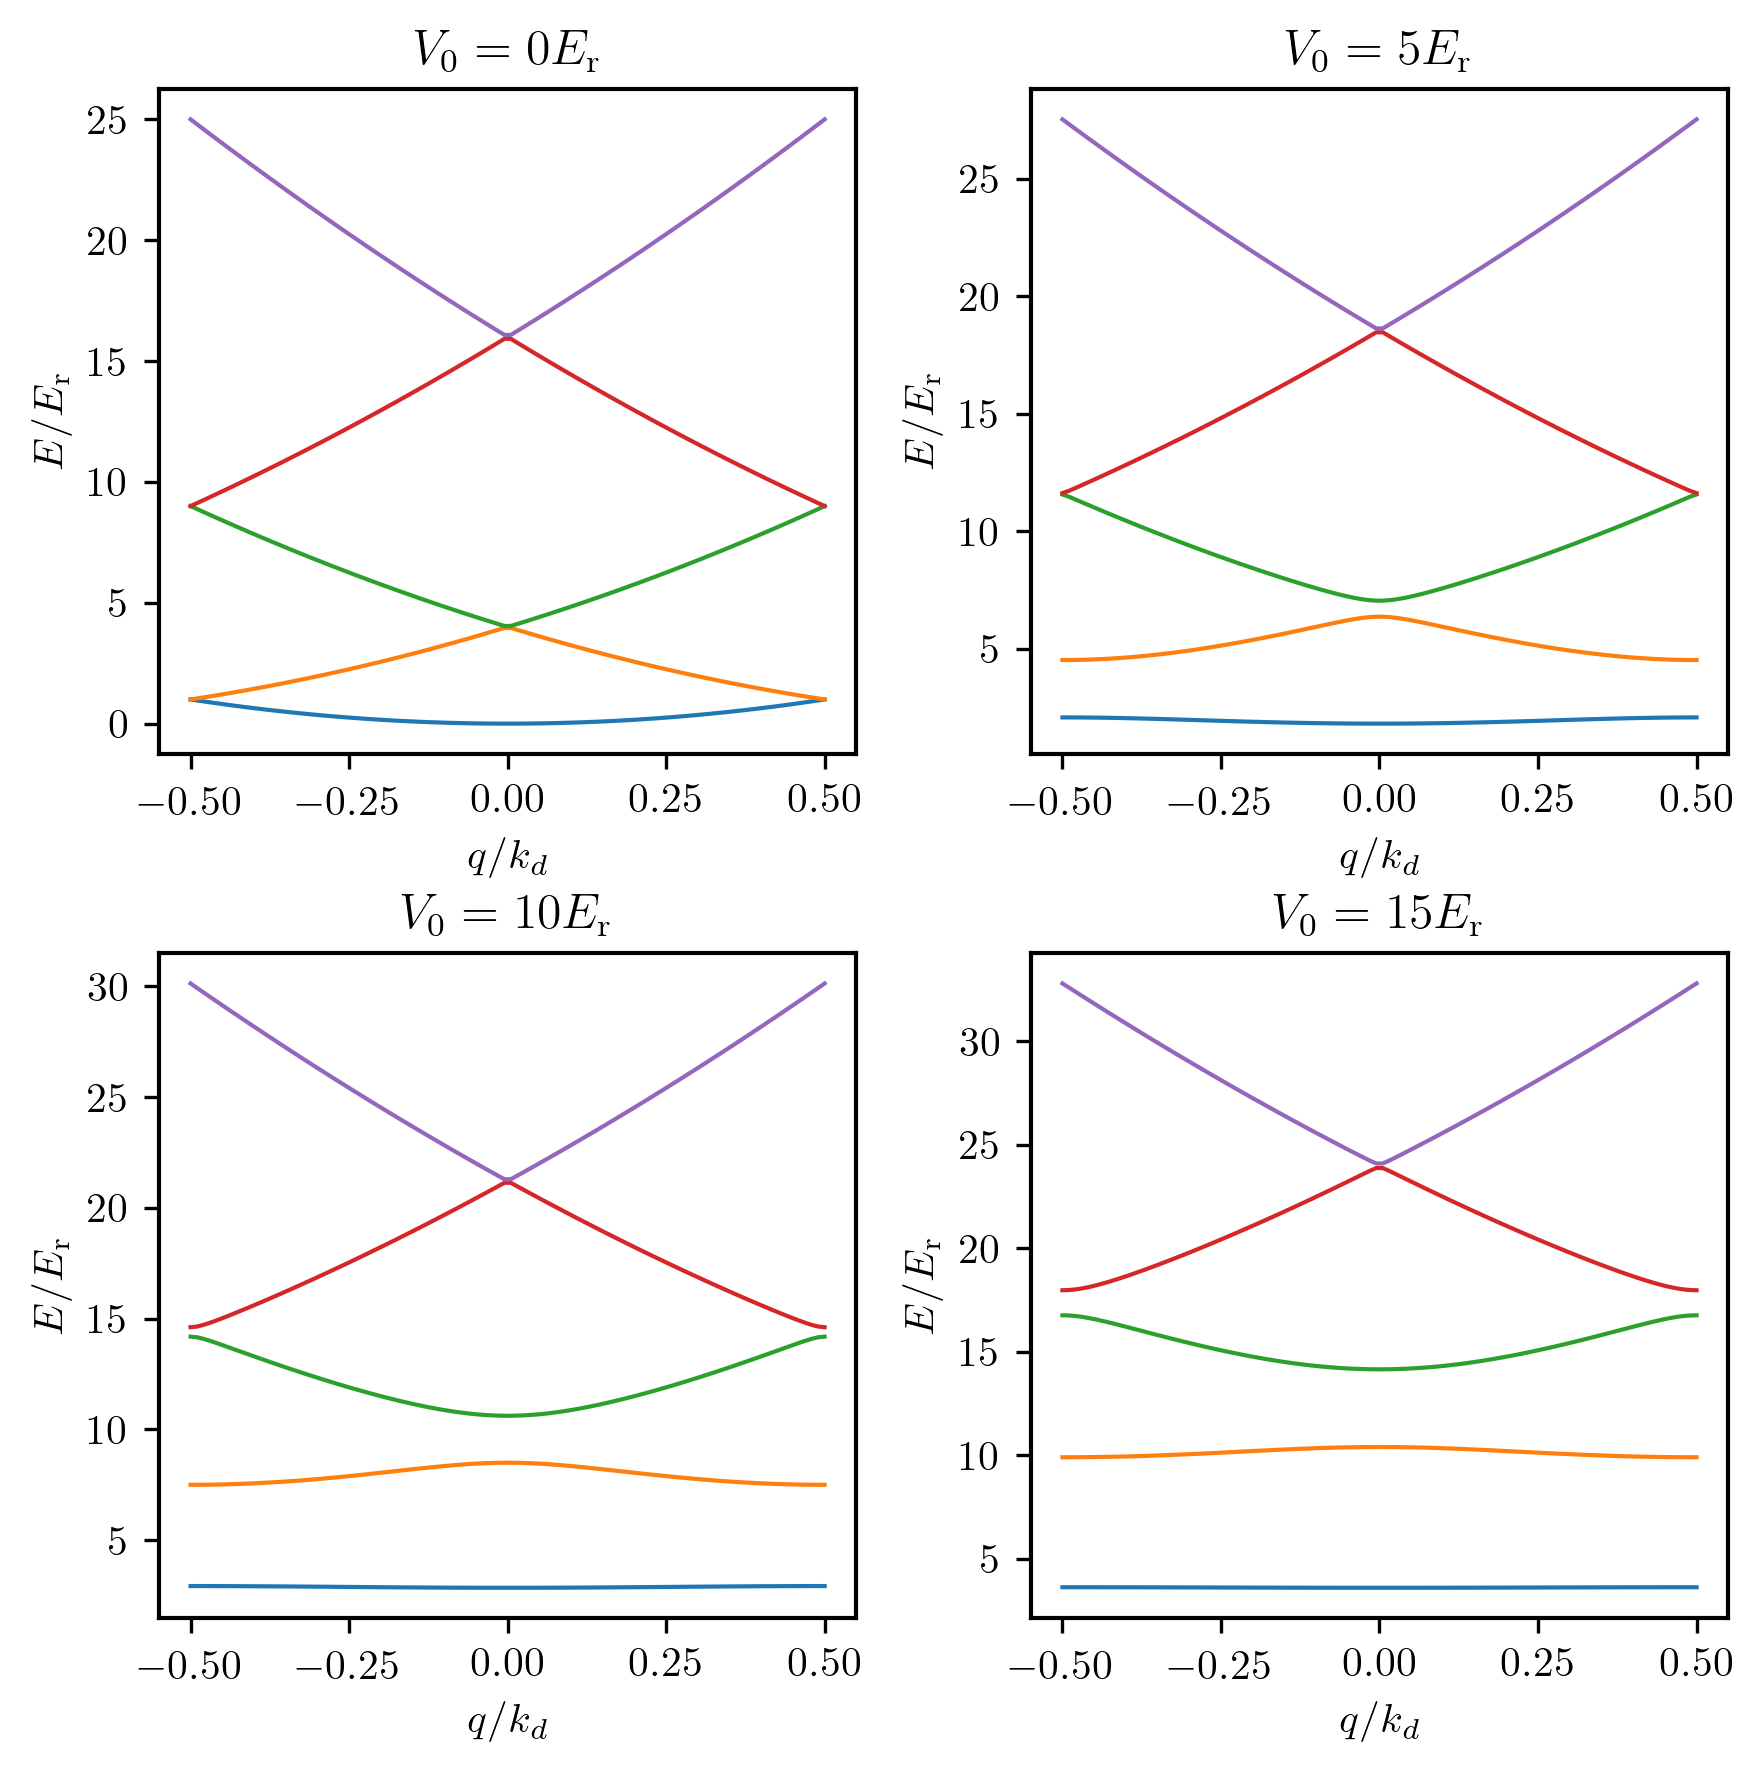
\includegraphics[width=\textwidth]{Fig/Chapter2/bloch_bands.png}
    \caption{First five Bloch energy bands for various lattice amplitudes $V_0$. The gap between the first bands increases as $V_0$ increases.}
    \label{fig:bloch_bands}
\end{figure}

In addition to the Bloch waves, it is possible to define a new kind of functions called the\textbf{ Wannier functions} \cite{wannier1937structure} that are localized near the lattice sites. They are defined from the Bloch waves by:

\begin{equation}
    w_{n, j}(x)=\sqrt{\frac{d}{2 \pi}} \int_{\mathrm{BZ}} \psi_{n, q}(x) e^{-i j q d} \mathrm{~d} q \quad, j \in \mathbb{Z}
    \label{eq:wannier_functions}
\end{equation}

\noindent with BZ denoting an integration over the first Brillouin zone and where $j$ can be interpreted as the index of a lattice site. Actually, we have from equation \ref{eq:wannier_functions} the simple relation:

\begin{equation}
    w_{n, 0}(x-j d)=w_{n, j}(x)
\end{equation}

The Bloch waves can then be re-written with the definition of the Wannier functions and write:

\begin{equation}
    \psi_{n, q}(x)=\left(\frac{d}{2 \pi}\right)^{1 / 2} \sum_{j} w_{n, j}(x) e^{-i j d q}
    \label{eq:bloch_as_wannier}
\end{equation}

The Bloch waves are then then sum of the localized Wannier function $w_{n, j}$ that can be interpreted as the wave-function of a particle located in lattice site $j$. The Hamiltonian of the system can also be re-written in terms of Wannier function. To do so, we start by writing it in the Bloch waves basis with the second quantification formalism, introducing the operator $\hat{c}_{n,q}$ that destroys a particle in the Bloch wave $\psi_{n,q}$.

\begin{equation}
    H_{1}=\sum_{n} \int_{\mathrm{BZ}} E_{n}(q) \hat{c}_{n, q}^{\dagger} \hat{c}_{n, q} \mathrm{~d} q
    \label{eq:H_bloch}
\end{equation}

To change into the Wannier function basis as defined in \ref{eq:bloch_as_wannier}, we introduce the operator $\hat{b}_{n,j}$ destroying a particle in the Wannier function $w_{n,j}$ and defined such as:

\begin{equation}
    \hat{c}_{n}(q)=\sqrt{\frac{d}{2 \pi}} \sum_{j} \hat{b}_{n, j} e^{i j d q}
    \label{eq:a_wannier}
\end{equation}

\noindent Injecting equation \ref{eq:a_wannier} in equation \ref{eq:H_bloch}, we get:

\begin{equation}
    H_{1}=\sum_{n} \sum_{j, j^{\prime}} J_{n}\left(j-j^{\prime}\right) \hat{b}_{n, j^{\prime}}^{\dagger} \hat{b}_{n,j}
    \label{eq:H_Jn}
\end{equation}

\noindent This Hamiltonian has a nice physical meaning: it describes the tunneling process by which a particle in site $j$ can ``hop'' to another lattice site $j'$ with the tunneling amplitude $J_n (j-j')$ that writes:

\begin{equation}
    J_{n}\left(j-j^{\prime}\right)=\frac{d}{2 \pi} \int_{\rm{BZ}} e^{i\left(j-j^{\prime}\right) q d} E_{n}(q) \mathrm{d} q
\end{equation}

\noindent The probability for a particle to tunnel from lattice site $j$ to $j'$ is reduced as the distance between the two sites $j$ and $j'$ increases and as the potential barrier, \ie the lattice amplitude increases.

We will focus ourselves on the ground-state properties of the system and therefore assume that the lowest energy band is the only populated. This assumption is valid as long as $V_0 \geq 2.2 \ E_{\rm{E_r}}$ at which the gap is opening. In addition, for $V_0 \geq 3 \ E_{\rm{E_r}}$, we can use the tight-binding approximation for which only the tunneling events between adjacent sites are non-negligible. We simplify the Hamiltonian \ref{eq:H_Jn} by replacing  $J_{n}\left(j-j^{\prime}\right)$ by a constant $J$ denoting the probability to tunnel between adjacent lattice sites that we define as:

\begin{equation}
    J=-J_0(1)
\end{equation}

\noindent so that $J$ is positive. Finally, we obtain the first term of the Bose-Hubbard Hamiltonian:

\begin{equation}
    \hat{H}_1 = -J \sum_{\mean{i,j}} \hat{b}^{\dagger}_i \hat{b}_j
    \label{eq:H_band}
\end{equation}

\noindent where $\mean{i,j}$ denotes the ensemble of all adjacent lattice sites $i$ and $j$.

\subsubsection{Interaction term}
We now turn to studying the interaction term that we had left out in the full Hamiltonian of equation \ref{eq:H_lattice_full}. In the formalism of second quantification, the short-range, $s$-wave, 3D interaction Hamiltonian writes:

\begin{equation}
    \hat{H}_{\mathrm{int}}=\frac{1}{2} \int d x \int d x' U_{\mathrm{int}}\left(x, x'\right) \hat{\Psi}^{\dagger}(x) \hat{\Psi}^{\dagger}\left(x'\right) \hat{\Psi}\left(x^{\prime}\right) \hat{\Psi}(x)
\end{equation}

\noindent with $\hat{\Psi}(x)$ the operator destroying a particle at position $x$ that we write in terms of Wannier functions as:

\begin{equation}
    \hat{\Psi}(x)=\sum_{j} w_{j}(x) \hat{b}_{j} = \sum_{j} w_{0}(x-x_j) \hat{b}_{j} 
    \label{eq:atom_operator_lattice}
\end{equation}

\noindent Note that we dropped the energy band number $n$ as we are studying the ground-state properties and thus only the lowest energy band. We approximate the interactions to be contact, repulsive interactions so that:

\begin{equation}
    U_{\rm{int}}= g \delta (x_1 - x_2)
\end{equation}

\noindent with $g$ the strength of the interactions. The interaction Hamiltonian can then be re-written:

\begin{equation}
    \hat{H}_{\mathrm{int}}=\frac{g}{2} \sum_{j_{1}} \sum_{j_{2}} \sum_{j_{3}} \sum_{j_{4}} \hat{b}_{j_{4}}^{\dagger} \hat{b}_{j_{3}}^{\dagger} \hat{b}_{j_{2}} \hat{b}_{j_{1}} \int w_{j_{4}}^{*}(x) w_{j_{3}}^{*}(x) w_{j_{2}}(x) w_{j_{1}}(x) \mathrm{~d} x
    \label{eq:h_int_intermediate}
\end{equation}

\noindent which is still a fairly complicated expression. We can however greatly simplify it by considering that the Wannier functions become narrower as the lattice depth increases. The overlap between the Wannier functions of the different lattice sites then becomes increasingly negligible. This means that the integral of equation \ref{eq:h_int_intermediate} is non zero only if $j_1=j_2=j_3=j_4$, \ie if we only consider on-site interactions. In the end, the interaction Hamiltonian writes:

\begin{equation}
    \hat{H}_{\rm{int}}=\frac{U}{2} \sum_j \hat{n}_j (\hat{n}_j -1)
\end{equation}

\noindent where we have introduced the on-site energy $U_{\mathrm{1D}}=g \int\left|w_{0,0}(x)\right|^{4} \mathrm{d}x$, easily generalized to the 3D case with $U=g \int(\left|w_{0,0}(x)\right|^{4} \mathrm{d}x)^3$. 

Combining this Hamiltonian to the non-interacting Hamiltonian of equation \ref{eq:H_band}, we reach the form of the famous \textbf{Bose-Hubbard Hamiltonian}:

\begin{equation}
    \hat{H}_{\mathrm{BH}}= -J \sum_{\mean{i,j}} \hat{b}^{\dagger}_i \hat{b}_j + \frac{U}{2} \sum_j \hat{n}_j (\hat{n}_j -1)
\end{equation}

\noindent Interestingly, the physics of the homogeneous ground-state depends on the two parameters $J$ and $U$ as we will see in the next paragraph. In particular, the ratio $U/J$ depends on the lattice depth $V_0$ that is easily controllable in an experiment, for instance by changing the power of the laser beams used to produce the lattice potential.


\section{The superfluid to Mott insulator transition}

We discuss in this section the properties of the Bose-Hubbard Hamiltonian ground-state for $N$ particles spread over $M$ sites, characterized by the ratio $U/J$ of the on-site interaction energy $U$ and the tunneling coefficient $J$. To begin, we describe the extreme cases $U/J \to 0$ and $U/J \to \infty$, which are the only cases for which the Hamiltonian can be analytically solved. 

\subsection{Extreme cases}

\subsubsection{Perfect superfluid (SF) phase $\bm{U/J \to 0}$}

In this case, the particles are non-interacting. In these conditions, the ground-state $\ket{\Psi_0}$ of the N particles system is simply the product of the single particle ground state wave-function, \ie the Bloch wave-function for $q=0$ \cite{bloch2008many}:

\begin{equation}
    \ket{\Psi_0}_{\mathrm{SF}} = \frac{1}{\sqrt{N!}} (\hat{c}^{\dagger}(\bm{q}=0))^N \ket{0} = \frac{1}{\sqrt{N !}}\left(\frac{1}{\sqrt{M}} \sum_{j=1}^{M} \hat{b}_{j}^{\dagger}\right)^{N} \ket{0}
\end{equation}

\noindent The ground-state is then an ideal Bose-Einstein condensate with a condensed fraction equal to 1. In the thermodynamic limit with $N \to \infty$, $M \to \infty$, and the average filling defined as $\bar{n}=N/M$, it is possible to show at the price of a few lines of complex calculations \cite{gerbier_notes} that the probability to find $n_i$ atoms at a given site $i$ is:

\begin{equation}
    p\left(n_{i}\right) \approx e^{-\bar{n}} \frac{\bar{n}^{n_{i}}}{n_{i} !}
\end{equation}

\noindent We recognize the same Poissonian distribution that we would obtain for a bosonic coherent state as described in Chapter \ref{sec:chapter_1}. We can therefore write:

\begin{equation}
    \ket{\Psi_0}_{\mathrm{SF}} \approx |\Psi\rangle_{\mathrm{coh}}=\mathcal{N} e^{\sqrt{N} \hat{c}^{\dagger}(\bm{q}=0)} \ket{0} = \mathcal{N} \prod_{i} e^{\sqrt{\bar{n}} \hat{b}_{i}^{\dagger}} \ket{0} = \prod_{i} \mathcal{N}_{i} \sum_{n_{i}=0}^{\infty} \frac{\alpha_{i}^{n_{i}}}{\sqrt{n_{i} !}}\left|n_{i}\right\rangle_{i}
\end{equation}

\noindent with $\alpha_i=\sqrt{\bar{n}} \ \forall i \in \Z$ and the normalization factor $\mathcal{N}_{i}=e^{-\left|\alpha_{i}\right|^{2} / 2}$. We thus find that the ground state can be described as a product of local coherent states associated to the different lattice sites.

As we did in Chapter \ref{sec:chapter_1}, we can write the first-order correlation function between two different lattice sites $i$ and $j$ to characterize the coherence properties of the ground-state:

\begin{equation}
    G^{(1)}(i,j)= \mean{\hat{b}^{\dagger}_i \hat{b}_j}
\end{equation}

\noindent In the limit $U \to 0$, $G^{(1)}(i,j)$ is easy to calculate and writes:

\begin{equation}
    G^{(1)}(i,j)= {}_{\mathrm{SF}} \bra{\Psi_0} \hat{b}^{\dagger}_i \hat{b}_j \ket{\Psi_0}_{\mathrm{SF}} = \alpha^*_i \alpha_j = \bar{n}
\end{equation}

We see that the result does not depend from the chosen lattice sites $i$ and $j$ and thus from the distance between them, indicating an infinite range coherence.


\subsubsection{Perfect Mott Insulator (MI) phase $\bm{U/J \to \infty}$}

In the opposite extreme limit, the tunneling probability goes to zero $J=0$ so that each of the lattice sites are independent from one another. The Hamiltonian reduces to:

\begin{equation}
    \hat{H}_{\mathrm{BH}} = \frac{U}{2} \sum_j \hat{n}_j (\hat{n}_j -1)
\end{equation}

Because of the strong repulsive interactions, the particle localize on the lattice sites and cannot hop from site to site as $J=0$. The ground-state is then reached by distributing the particles among the different sites of the lattice so that the number of particles per site is as low as possible to minimize the interaction energy. This corresponds to putting $\bar{n}=N/M$ particles in each of the $M$ available lattice sites. The ground-state then has the simple expression of a Fock state:

\begin{equation}
    \left|\Psi_{0}\right\rangle_{\mathrm{MI}}=\frac{1}{\sqrt{N !}} \prod_{j=1}^{M}\left(\hat{b}_{j}^{\dagger}\right)^{\bar{n}}|0\rangle
\end{equation}

\noindent This state is called the \textbf{Mott insulator} state \cite{fisher1989boson}. The first-order correlation function now writes

\begin{equation}
     G^{(1)}(i,j)= {}_{\mathrm{MI}} \bra{\Psi_0} \hat{b}^{\dagger}_i \hat{b}_j \ket{\Psi_0}_{\mathrm{MI}} = \delta_{i,j}
\end{equation}

\noindent and is zero when we consider any pair of different lattice sites with $i \neq j$. In the limit $J \to 0$, the system is therefore incoherent.

\subsection{The $T=0$ Mott phase transition}

What can then be said from intermediates values of $U/J$? If we start from the case $J=0$ and progressively start increasing $J$, it becomes possible for the atoms to hop from site to site. When an atom hops to an adjacent site, the occupancy is increased, increasing the energy by $U$. When the gain in kinetic energy $J$ is smaller than $U$, this process is unfavorable and the atoms remain localized on the lattice sites. However, when $J$ is larger than $U$, the gain in kinetic energy outweighs the effect of the interactions and the atoms hop through the different sites of the lattice. The ground-state of the Bose-Hubbard then undergoes a phase transition as $U/J$ varies from an \textbf{insulating phase} to a \textbf{superfluid phase} with very different properties.

\begin{minipage}[t]{0.45\textwidth}
    \noindent \textbf{Superfluid phase}
    \begin{itemize}
        \item The atoms are delocalized over the entire lattice.
        \item The condensed fraction is non zero.
        \item The system shows long range coherence, \ie the phase is fixed.
        \item The on-site number of atoms is fluctuating.
        \item For low values of $U/J$ far from the transition, the effect of interaction is small, meaning that the fraction of atoms populating the quasi-momenta $q$ outside of the BEC is small as well. As in Chapter \ref{sec:chapter_1}, we can use the Bogoliubov approximation to find that the excitation spectrum is gapless and phonon-like at low $q$.
    \end{itemize}
\end{minipage}
\begin{minipage}[t]{0.48\textwidth}
    \noindent \textbf{Insulating phase}
    \begin{itemize}
        \item The atoms are well localized on the lattice sites.
        \item The condensed fraction is zero.
        \item The system is incoherent, the phase is fluctuating.
        \item The on-site number of atoms is well defined and non fluctuating.
        \item The excitation spectrum is gapped, with the excitations consisting of particle-hole modes that can restore short-range coherence. 
    \end{itemize}
\end{minipage}

\subsubsection{Phase diagram}

To discuss the location of the critical point $(U/J)_c$, we slightly complexify our model where we had only considered commensurate fillings, \ie when $\bar{n}=n_0$ with $n_0$ an integer, thus fixing the chemical potential that we now set to be a free parameter. We plot on Fig.-\ref{fig:mott_lobes} the full phase diagram function of $\mu/U$, set by the filling in the Mott insulator phase $\bar{n}$ and $J/U$. As the system is homogeneous, the filling $\bar{n}$ is independent of $U/J$. The grey dashed lines correspond to iso-filling lines for a given value of $\bar{n}$. For commensurate fillings, the iso-filling lines cross the Mott stability lobes at the critical ratio $(U/J)_c$ that increases ad the filling increases. If the filling is however incommensurate (line $n=1+\varepsilon$), we notice that the system remains in the superfluid phase as long as $J \neq 0$. This is due to the fact that a small fraction of the atoms can delocalize over the whole lattice without being blocked by the interactions $U$ as there will never be two of these particles in the same site as a consequence of the fact that the filling is incommensurate.

\begin{figure}
    \centering
    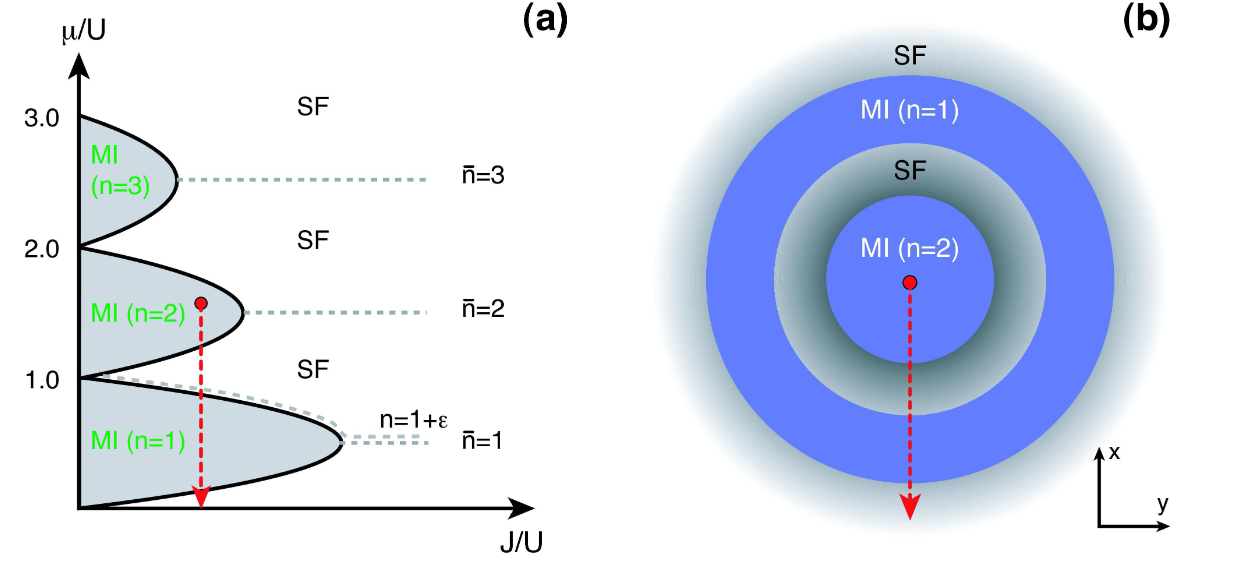
\includegraphics[width=0.9\textwidth]{Fig/Chapter2/mott_lobes.png}
    \caption{a) Homogeneous phase diagram as a function of $\mu/U$ and $J/U$. The dashed lines are iso-filling lines. We observe a Superfluid to Mott Insulator phase transition for commensurate fillings. b) Wedding-cake structure for the trapped gas. The red arrow illustrate how $\mu_{\rm{eff}}$ varies and the corresponding phases as the distance from the center of the trap increases. Taken from \cite{bloch2008many}.}
    \label{fig:mott_lobes}
\end{figure}


\subsection{Trapping effects}

In practice, the system is not homogeneous as we require an external harmonic potential $V_{\rm{ext}}(\bm{r})$ to trap the atoms for experiments. The properties of the trapped system can be linked to the properties of the homogeneous system by applying the Local Density Approximation\footnote{Valid as long as the trapping potential varies slowly from site to site and the system is at thermal equilibrium. This approximation may however fail at the quantum critical point \cite{pollet2012recent}.} \cite{bergkvist2004local} and replacing the chemical potential by an effective one:

\begin{equation}
    \mu_{\rm{eff}}= \mu - V_{\rm{ext}}(\bm{r})
\end{equation}

\noindent This means that the chemical potential, and thus the lattice filling, varies with the distance from the center of the trap. A typical situation is illustrated by the red arrow on the phase diagram of Fig.-\ref{fig:mott_lobes} where $J/U$ is small enough for Mott phases to exist and the center of the trap corresponds to a filling $\bar{n}=2$. As we get away from the center of the trap towards regions of low $\mu_{\rm{eff}}$ following the red arrow, we exit the first Mott region $\bar{n}=2$ to enter a superfluid region where the filling decreases continuously up to a second Mott region with filling $\bar{n}=1$ and finally reach a last superfluid region at the edge of the trap at vanishing values of $\mu_{\rm{eff}}$. The Mott phases are incompressible, meaning that the density remains constant even though the external trapping potential is rising, differentiating them from the superfluid region. This results in the famous ``wedding-cake'' density profile as illustrated on panel b) of Fig.-\ref{fig:mott_lobes}.

\noindent For clarity sake, the system will be said to be in the Mott Insulator phase as long as a Mott plateau exists, \NOTE{finir cette phrase}

\subsection{Finite temperature effects}

If we finally consider the effect of temperature, we obtain the complete phase diagram of Fig.-\ref{fig:phase_diagram} function of $T/J$ and $U/J$ with the apparition of a additional phase, the normal (thermal) gas. For $U/J \leq (U/J)_c$, the superfluid phase undergoes a condensation transition with temperature similar to the well-known BEC transition. This transition is induced by the thermal fluctuations and is then called classical, in opposition to the Mott transition which is a quantum phase transition \NOTE{finir}. On the other hand, the Mott insulator phase also goes to the normal gas phase as the temperature increases, but with a smooth crossover. Interestingly, the Superfluid to Mott Insulator transition subsists at low temperature. The green area indicates the Quantum Critical Region for which we expect the critical quantum effects of the Mott transition to survive in spite of the temperature.

\begin{figure}
    \centering
    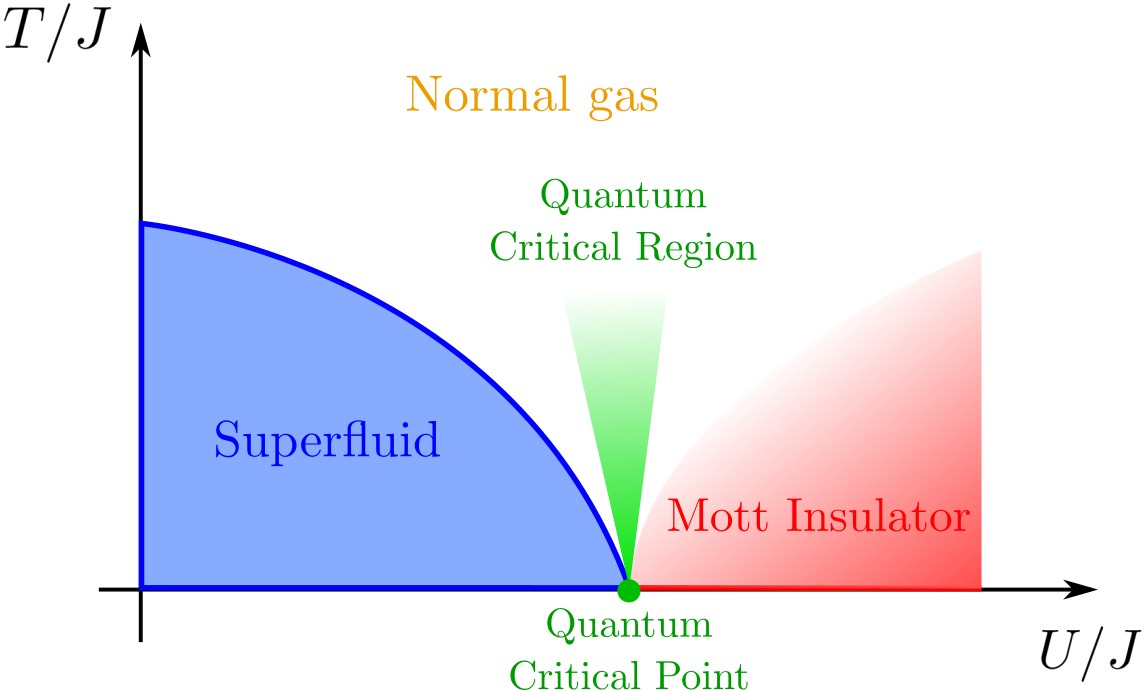
\includegraphics[width=0.78\textwidth]{Fig/Chapter2/phase_diagram.png}
    \caption{Bose-Hubbard phase diagram function of $T/J$ and $U/J$. We identify three phases, the Superfluid, Mott Insulator, and Normal Gas. The green area indicates the region in which critical point quantum effects could be observable in spite of the finite temperature.}
    \label{fig:phase_diagram}
\end{figure}



\section{Accessing the in-trap momentum distribution}

Now that we have laid down the main elements of lattice gases physics, we need to determine how to experimentally study them \NOTE{pas terrible}. As developed in Chapter \ref{sec:chapter_1}, our main focus will be on the \textbf{momentum space} correlations, requiring us to devise a technique to effectively measure the momentum distribution of a lattice gas. The most natural idea for momentum space measurements is to use the well-known and widely used \textbf{Time-Of-Flight} (TOF) technique. This technique consists in suddenly turning off the trapping potential to let the atoms fall under the effect of gravity and measure their positions $\bm{r}$ after a given Time-Of-Flight $t_{\rm{TOF}}$. In a very simple picture with classical and non-interacting particles, this position gives information about the in-trap momentum of the particle through the simple \textbf{ballistic relation}:

\begin{equation}
    \hbar \bm{k} = \frac{m \bm{r}}{t_{\rm{TOF}}}
\end{equation}

The validity of this simple relation is however far from being obvious for gases released from optical lattice. We will then describe in this section the TOF dynamics of an atomic gas released from an optical lattice to identify the conditions under which a TOF measurement can be properly used to measure the in-trap momentum of the gas.

% \subsection{The momentum distribution}

% The momentum distribution of a gas of atoms on a homogeneous lattice writes \cite{gerbier2008expansion}:

% \begin{equation}
%     n(\mathbf{k}) \propto |\tilde{w}(\mathbf{k})|^{2} \sum_{i,j} e^{i \mathbf{k} \cdot (\bm{r}_i - \bm{r}_j)} G^{(1)}(i,j)
% \end{equation}

% \noindent where $\tilde{w}(\mathbf{k})$ denotes the Fourier transform of the single site Wannier function. The momentum distribution is thus strongly dependent from the lattice depth. For $U/J \to 0$, $G^{(1)}(i,j) = \bar{n}$ meaning that the momentum distribution consists of sharp peaks located at $k = j k_d$ with $j \in \Z$. In the other limit $U/J \to \infty$, $G^{(1)}(i,j) = \delta_{i,j}$ so that the momentum distribution reduces to $|\tilde{w}(\mathbf{k})|^{2}$, \ie a Gaussian-like function.

\subsection{Expansion from the lattice and Far Field regime}

We start our calculations with the simplified case for which we neglect the effects of all interactions during the TOF. In this configuration, the problem is very similar to the diffraction of a light wave by a grating in optics. The diffraction interference pattern results from the coherent sum of the contribution of many source points associated to each of the diffraction grating holes. For the lattice gas, the source points correspond to the lattice sites associated to Wannier functions that will be able to interfere if the system is coherent. For simplicity sake, we will only consider the 1D case for which the 3D case can be easily obtained as the non-interacting Hamiltonian is separable.

At time $t=0$, right before the lattice potential is turned off, the atomic field operator writes (see \ref{eq:atom_operator_lattice})

\begin{equation}
    \hat{\Psi}(x)= \sum_{j} w_{0}(x-x_j) \hat{b}_{j} 
    \label{eq:field_operator}
\end{equation}



The expression of the Wannier functions is rather complex and very hard to handle in calculations. However, we can approximate the lattice potential near a minimum to its second-order Taylor expansion, \ie approximate it to a harmonic potential of frequency $\omega_L=2 \sqrt{s} (E_{\rm{r}}/\hbar)$ \cite{toth2008theory}. As illustrated in \NOTE{faire figure}, this means that the Wannier function can be well approximated by the Gaussian wave-function of the harmonic oscillator ground state:

\begin{equation}
    w_0(x) \simeq \frac{1}{\pi^{1 / 4} \sqrt{x_{0}}} \exp \left(\frac{-x^{2}}{2 x_{0}^{2}}\right)
\end{equation}

\noindent with $x_{0}=\sqrt{\hbar / m \omega_{l}}$.

When the lattice potential is turned off, each of the lattice sites wave-functions expand freely following the harmonic oscillator dynamics \cite{toth2008theory}:

\begin{equation}
    w\left(x-x_{j}, t\right)=\frac{1}{\pi^{1 / 4} \sqrt{W(t)}} \exp \left(-\frac{\left(x-x_{j}\right)^{2}}{2 W(t)^{2}}\right) \exp \left(-i \frac{\left(x-x_{j}\right)^{2}}{2 W(t)^{2}} \frac{h t}{m x_{0}^{2}}\right)
    \label{eq:time_dependent_wannier}
\end{equation}

\noindent with $W(t)=x_{0} \sqrt{1+\left(\hbar t / m x_{0}^{2}\right)^{2}}$ the width of the Gaussian envelope.

\subsubsection{The Far-Field regime}

In practice, as $\omega_L$ is high ($\sim 10^5-10^6 \ \rm{Hz}$), $W(t)$ increases very quickly. For instance, with $s=5$, $W(t)$ is multiplied by $\sim 600$ after $1 \ \rm{ms}$ of expansion and is thus much larger than the size of the lattice $L$. For $t>1 \ \rm{ms}$, we can make the approximation $W(t) \simeq \hbar t/m x_0$ as well as neglect the dependency on the initial site $x_j$ in the amplitude term as long as $|x| \ll W(t)$ so that we can write:

\begin{equation}
    \exp \left(-\frac{\left(x-x_{j}\right)^{2}}{2 W(t)^{2}}\right) \simeq \exp \left(-\frac{x^{2}}{2 W(t)^{2}}\right)
\end{equation}

\noindent This is equivalent to the paraxial approximation of the Fraunhofer diffraction regime.

Building up on the diffraction analogy, we would like to define an analog Fraunhofer distance where the dependency of the phase factor on the quadratic analog Fresnel term in $x_j$ can be neglected. Using $W(t) \simeq \hbar t/m x_0$, we obtain $\frac{\left(x-x_{j}\right)^{2}}{2 W(t)^{2}} \frac{h t}{m x_{0}^{2}} \simeq \frac{\left(x-x_{j}\right)^{2}}{2 x_0 W(t)}$ from which we derive the condition $\frac{x_j^2}{2 x_0 W(t)} \ll 1, \forall j$ that we rewrite \cite{gerbier2008expansion,toth2008theory}:

\begin{equation}
    t \gg t_{\rm{FF}} = \frac{mL^2}{2 \hbar}
\end{equation}

\noindent This condition defines the \textbf{Far-Field regime} after which the interference pattern is well resolved, in analogy to the Fraunhofer regime of diffraction. Combining the different approximations, we simplify \ref{eq:time_dependent_wannier} to:

\begin{equation}
    w\left(x-x_{j}, t\right)=\sqrt{\frac{m}{\hbar t}} \tilde{w_0}[Q(x,t)] \exp\left(-i \frac{\hbar Q(x,t)^{2}}{2 m} \right) \exp\left(i Q(x,t) x_{j}\right)
\end{equation}

\noindent with $Q(x,t)=\frac{m x}{\hbar t}$ and $\tilde{w_0}$ the Fourier transform of the Wannier function. 

Now that we have the general expression of $w\left(x-x_{j}, t\right)$, we generalize it to the 3D case and inject it in equation \ref{eq:field_operator} to obtain the sum of the contribution of each site:

\begin{equation}
    \hat{\Psi} (\bm{r},t) = \left(\sqrt{\frac{m}{\hbar t}} \right)^3 \tilde{w}[\bm{Q}(\bm{r},t)] \exp\left(-i \frac{\hbar \bm{Q}(\bm{r},t)^{2}}{2 m} \right) \sum_j e^{i \bm{Q}(\bm{r},t). \bm{r}_{j}} \hat{b}_j
\end{equation}

\noindent From this expression, we finally obtain the atomic density $\rho_{\rm{TOF}}(\bm{r},t) = \mean{\hat{\Psi} (\bm{r},t), \hat{\Psi}^{\dagger} (\bm{r},t)}$ at position $\bm{r}$ and a long TOF $t$:

\begin{equation}
    \rho_{\rm{TOF}}(\bm{r},t) = \left(\frac{m}{\hbar t} \right)^3 |w_0(\bm{Q}(\bm{r},t))|^2 \sum_{i,j} e^{i \bm{Q}(\bm{r},t).(\bm{r}_j - \bm{r}_{i})} \mean{\hat{b}^{\dagger}_i \hat{b}_j }
    \label{eq:rho_tof}
\end{equation}

\noindent The density $\rho_{\rm{TOF}}(\bm{r},t)$ then consists of a smooth envelope $|w_0(\bm{Q}(\bm{r},t))|^2$ set by the Fourier transform of the Wannier function and an interference term $\sum_{i,j} e^{i \bm{Q}(\bm{r},t).(\bm{r}_j - \bm{r}_{i})} \mean{\hat{b}^{\dagger}_i \hat{b}_j }$ that characterizes the coherence properties of the system. 

\subsubsection{Relation to the momentum distribution}

The main purpose of the TOF technique is to obtain information on the momentum distribution of the gas. To this end, we must find the relation between the measured quantity $\rho_{\rm{TOF}}(\bm{r},t)$ and the in-trap momentum distribution $\rho(\bm{k})$. To do so, we introduce the operator $\hat{a}_{\bm{k}}$ destroying a particle in mode $\bm{k}$:

\begin{equation}
    \hat{a}_{\bm{k}}=\frac{1}{\sqrt{V}} \sum_{j} e^{i \bm{k} \cdot \bm{r}_{j}} \hat{b}_{j}
\end{equation}

\noindent where $V$ is the quantization volume set to be the in-trap volume of the gas. The momentum density then writes:

\begin{equation}
    \rho(\bm{k})=\left\langle\hat{a}^{\dagger}_{\bm{k}} \hat{a}_{\bm{k}}\right\rangle=\frac{1}{V} \sum_{j, i} e^{-i \bm{k} \cdot\left(\bm{r}_{j}-\bm{r}_{i}\right)}\left\langle\hat{b}_{i}^{\dagger} \hat{b}_{j}\right\rangle
    \label{eq:momentum_distribution}
\end{equation}

\noindent If the particle are non-interacting, the ballistic relation gives $\bm{k} = m \bm{r}/\hbar t_{\rm{TOF}}$. From equation \ref{eq:rho_tof}, we obtain:

\begin{equation}
    \rho(\bm{k}) = \frac{\rho_{\rm{TOF}}(\bm{r}=\hbar t\bm{k}/m,t)}{V  \left(\frac{m}{\hbar t} \right)^3 |w_0(\bm{k})|^2}
\end{equation}

In conclusion, under the conditions that there are no interactions during the TOF and $t_{\rm{TOF}} \gg t_{\rm{FF}}$ to be in the far-field regime, the TOF distribution maps the in-trap momentum distribution. 

\subsubsection{Momentum distribution across the Mott transition}

As we have just seen, the momentum distribution is strongly dependent from the coherence properties of the system and in turn of the lattice depth.

\begin{itemize}
    \item In the superfluid phase $U/J \to 0$, the system is coherent $G^{(1)}(i,j) = \bar{n}$. From equation \ref{eq:momentum_distribution}, we get that the momentum distribution consists of sharp analog diffraction peaks located at $\bm{k} = j k_d \bm{e}_i$ with $j \in \Z$ and $\bm{e}_i$ the unitary vector in direction $i=x,y,z$. In terms of $\rho_{\rm{TOF}}(\bm{r},t)$, the amplitude of the different peaks is set by the Fourier transform of the Wannier function. 
    
    \item In the Mott insulator phase $U/J \to \infty$ the system is totally incoherent $G^{(1)}(i,j) = \delta_{i,j}$. The momentum distribution is then constant, meaning that $\rho_{\rm{TOF}}(\bm{r},t)$ simply reflects the Fourier transform of the Wannier function, \ie a Gaussian-like function.
    
    \item For intermediate values of $U/J$, the visibility of the interference pattern progressively decreases as $U/J$ increases. In addition, as $V_0$ increases, the Wannier function is more and more localized so that the width of its Fourier transform increases. As a result, the population of the diffracted peaks increases with the lattice depth.
\end{itemize}

The experimental quantity $\rho_{\rm{TOF}}(\bm{r},t)$ is therefore a powerful tool to characterize the phase of the system across the Mott transition. This is illustrated on Fig-\ref{fig:mott_greiner} of the first experimental observation of the Mott transition with cold atoms \cite{greiner2002quantum}, on which we can clearly see the visibility decreasing with $V_0$.

Importantly, a characteristic of the Superfluid to Mott insulator transition is that even though the system is incoherent in the insulating phase, the coherence can be restored by ramping down the lattice depth to the superfluid phase. The standard procedure to characterize the presence of the Mott transition is then to set $V_0$ to be in the superfluid region, ramp up it up to see that the interference pattern disappear, and ramp it down to find back the interference pattern. This allows to certify that the loss of coherence is indeed an effect of the competition between $U$ and $J$ and not an experimental defect, such as unwanted heating of the cloud.

\begin{figure}
    \centering
    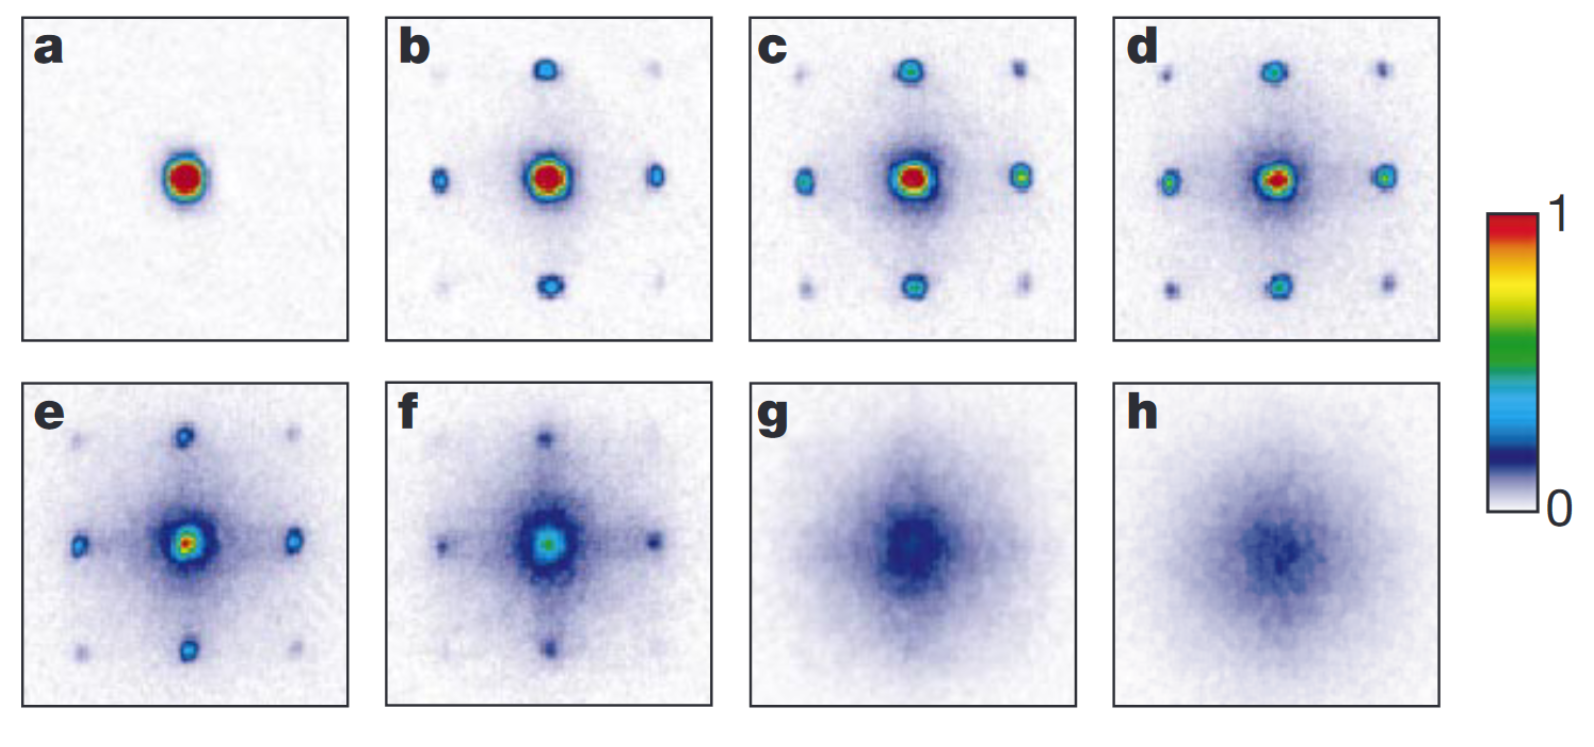
\includegraphics[width=0.9\textwidth]{Fig/Chapter2/mott_greiner.png}
    \caption{Absorption images of Rubidium atoms taken $15 \ \rm{ms}$ after the atoms are released from a 3D cubic lattice. Note that the far-field regime condition is not fulfilled here. \textbf{a)} s=0. \textbf{b)} s=3. \textbf{c)} s=7. \textbf{d)} s=10. \textbf{e)} s=13. \textbf{f)} s=14. \textbf{g)} s=16. \textbf{h)} 20. Taken from \cite{greiner2002quantum}.}
    \label{fig:mott_greiner}
\end{figure}


\subsection{Mean-field interactions}

\subsection{Beyond mean-field interactions}

